\section{Motivation}
\label{intro}

The modeling and the synthesis of online-reactive multi-action sequences
are important topics both in computer graphics and in humanoid robotics.
The most challenging part of the online control of complex whole-body behaviors is the coordination of the different tasks.

In the current work we present a novel approach that combines the walking pattern generator (WPG) presented in Chap.~\ref{chap:nmpc},
with an online kinematic planning architecture for full-body movements.
The upper body motion pattern generator is based on learned dynamical movement primitives.
And the lower body motion generator is based on model predictive control.
The approach is suitable for the online planning and control of reactive behaviors that integrates locomotion and reaching.
It also includes highly flexible re-planning even in short time horizons.
The locomotion planned by the WPG is combined with the planned motion of the upper body using the dynamic filter presented in An.~\ref{an:dyn:filter}.
This ensures that the overall behavior results in a dynamically stable gait with the predefined CoM velocities and predefined upper body motion.
The proposed method is characterized by a much smaller computational complexity than a direct motion planning using complex dynamical model.
The global computational complexity can be compared with the one of standard WPG algorithms \cite{herdt:ar:2010}.

\section{Related work}
\label{relatedworks}

The general problem of motion generation in a dynamic environment is challenging.
The continuous change of the environment and error in state estimations implies a relatively high control frequency, typically at least 10 HZ.
It also implies a reasonable preview horizon duration, typically at least $2$ steps or around $1.6\,s$ for a human size robot.
Solving a model predictive control problem for a humanoid robot with $30$ degrees of freedom in a horizon of $1.6\,s$ is still an open issue.
This implies that a priori knowledge or approximation of the problem lowering the complexity is needed.

Current solutions range from near real-time whole body Model Predictive Control with
regularized modeling of contacts in order to decrease the associated computational cost
\cite{tassa:iros:2012,Koenemann:iros:2015}.
To a precise modeling of contact phases, which requires hours of offline computation time \cite{ref:km12}.

Another challenging issue for the generation of human-like behaviors is the sequential planning of
multi-step sequences, where individual steps can be associated with different
sub-goals or constraints (like contact with goal objects or step-length constraints).
This problem being multidisciplinary, we quickly review associated work in computer graphics, biological motor control, and humanoid robotics.

\subsection{Modeling of whole-body movements in computer graphics}
The problems of kinematic synthesis of such complex whole body movements has been addressed
extensively in computer graphics, e.g. \cite{ref:lwhpk12}, and many learning-based approaches
have been proposed that provide low-dimensional parametrization of classes of whole body motion \cite{ref:wfh08}. Recently, more attention has been given
to  methods for the blending of learned motion primitives, whose concatenations over time have to
satisfy  additional task constraints.  For example, in \cite{ref:fxs12} captured motion samples were
blended exploiting a prioritized 'stack of controllers'. In \cite{ref:smkb14} the
instantaneous blending weights of controllers were prioritized by their serial order.
In \cite{ref:hk14} the coordination between locomotion and arm pointing in the
last step was modeled by blending and selecting arm pointing primitives dependent
on the gait phase.

\subsection{Biological motor control of multi-step sequences}
Human motor behavior including action sequences has been shown to be highly predictive.
This has been investigated, for example, in a recent study on the coordination of walking
and reaching \cite{ref:lrss13}. Human subjects had to walk towards a drawer and to
grasp an object, which was located at different positions in the drawer. Participants
optimized their behavior already multiple steps before the object contact, consistent with the
hypothesis of \emph{maximum end-state comfort} during the reaching action \cite{ref:ws10, ref:r08}.
This means that the steps prior to the reaching were modulated in a way that optimizes the distance
for the reaching action \cite{ref:lrss13}. In  \cite{ref:mlsg15} our partners have proposed a
learning-based framework that is based on movement primitives that are learned from motion capture data,
and which reproduces these human planning strategies for an application in computer animation.
The underlying architecture is simple and approximates complex full-body movements by
dynamic movement primitives that are modeled by nonlinear dynamical systems. These primitives
are constructed from kinematic primitives that are learned from trajectory sets by anechoic demixing.
Similar to  related approaches in robotics \cite{ref:gam08,ref:buc06}, the method generates complex
movements by the combination of a small number of learned dynamical movement primitives. Our partners have previously
demonstrated the advantages of this approach for the adaptive online generation of multi-step sequences
with coordinated arm movements \cite{ref:mlsg15, ref:gie09}.

\subsection{Related approaches in humanoid robotics}
Several  approaches have  been proposed in robotics for the synthesis of
walking combined with grasping movements. Indeed, the DARPA robotic challenge
valve manipulation task forced the researchers to find efficient and robust methods
to perform reaching and manipulation tasks. \cite{ref:Ajoudani2013} proposed
a hybrid controller, where the robot is using a goal-driven fast foot step planner in combination
with visual servoing for the reaching and grasping of the valve.
\cite{ref:kuindersma2015optimization} proposes
a complete control architecture for the humanoid robot Atlas that is able to localize the robot
and automatically finds foot step around or over obstacles in order to reach a user defined goal.
The architecture contains also a whole-body controller which allow the robot to get
up from a lying down position, or to do complex task like turn the valve.
Another team (IHMC) presented an architecture in \cite{ref:johnson2015team} with a more sophisticated
control of the locomotion in \cite{ref:Englsberger2015}.
All three mentioned control architectures can make a humanoid robot reach, and then
grasp or manipulate objects as required for the robotic challenge.
To our knowledge an online simultaneous coordination of both tasks has not been demonstrated so far.
Other solutions for the combination of walking and vision-controlled reaching of a static and mobile target during walking were proposed in \cite{ref:svdmsvey08} and \cite{ref:bjkeht13}.

Randomized motion planning methods allow the generation of complex whole body motion  in constrained environment but at a high computational cost \cite{ref:dklntl13,ref:kly11}.
\cite{ref:gtg10}  proposed an algorithm for the computation
of optimal stance locations with respect to the position of a reaching target, where a dynamical systems
approach was used to generate the reaching behavior.
\cite{yoshida2007give} used a task priority approach,
based on a  generalized inverse kinematics, in order to organize several sub-tasks, including stepping, hand motion,
and gaze control.
Other work has exploited global path planning in combination with walking pattern generators (WPGs) \cite{Kajita:icra:2003} in order to generate collision-free dynamically stable gait paths.

A first attempt to transfer human reaching movements to humanoid robots by using motion-primitives was proposed in
\cite{ref:ttsg13}. In this work the primitives were extracted by using PCA and the behavior was successfully
implemented on the HRP-2 robot, only involving the trunk and arm joints.
The use of motion primitives in robotics
was also proposed in \cite{ref:gnzwiau13}, also including the integration of force-feedback.
\cite{ref:inhps13} and \cite{ajallooeian_general_2013} proposed systems based on dynamical movement primitives that
can be  modulated in real-time for the generation of complex movements.
However their approach focus on learning the in an efficient way the input data.
In \cite{ref:inhps13} the transfer to robot is tackled by using a low level torque controller managing the feasibility of the system.
This could result in a different motion than the one learned.
So the transfer from balanced human locomotion to balanced robot locomotion is still an open question.

\section{System architecture}
\label{sc:SystemArchitecture}

\begin{figure}[ht]
\centering
\newcommand{\picturefontsize}{\LARGE}
\newcommand{\pictureLineWidth}{0.8mm}

% For every picture that defines or uses external nodes, you'll have to
% apply the 'remember picture' style. To avoid some typing, we'll apply
% the style to all pictures.
\tikzstyle{every picture}+=[remember picture]
\tikzstyle{na} = [baseline=-.5ex]

\def\localarrow{
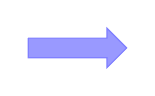
\begin{tikzpicture}
\path[draw=blue!50,fill=blue!40] (0,0.125) -- (1.0,0.125) -- (1.0,0.25) -- (1.25,0.0) -- (1.0,-0.25) -- (1.0,-0.125) -- (0.0,-0.125) -- (0.0,0.125);
\end{tikzpicture}
}

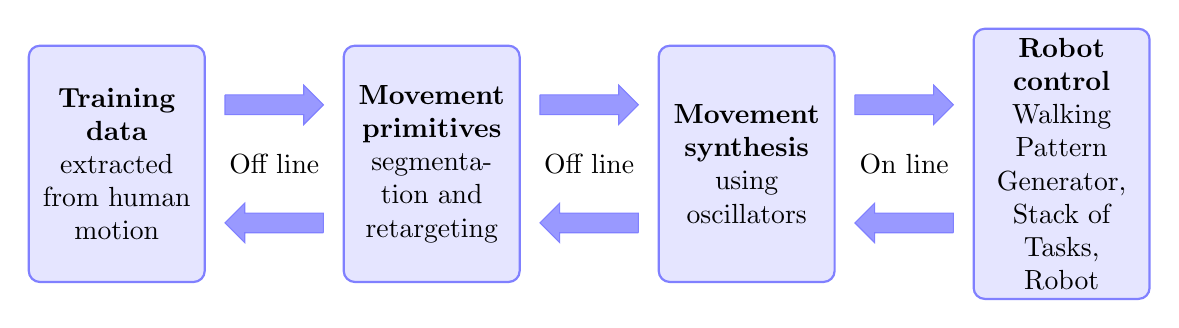
\begin{tikzpicture}%[show background grid]% every node/.style={draw,outer sep=0pt,thick}]

% Rectangle
\node (trainingdata) [text centered, shape=rectangle,rounded corners,draw=blue!50,fill=blue!10,thick,text width=2cm, minimum height=3cm]
  at (0.0,-0.5) {\textbf{Training data} extracted from human motion};

\node (movementprimitives) [text centered, shape=rectangle,rounded corners,draw=blue!50,fill=blue!10,thick,text width=2cm, minimum height=3cm]
  at (4.0,-0.5) {\textbf{Movement primitives} segmentation and retargeting};

\node (movementsynthesis) [text centered, shape=rectangle,rounded corners,draw=blue!50,fill=blue!10,thick,text width=2cm, minimum height=3cm]
  at (8.0,-0.5) {\textbf{Movement synthesis} using oscillators};

\node (robotcontrol) [text centered, shape=rectangle,rounded corners,draw=blue!50,fill=blue!10,thick,text width=2cm, minimum height=3cm]
  at (12.0,-0.5) {\textbf{Robot control}\\Walking Pattern Generator,\\ Stack of Tasks,\\ Robot};

\node (firstarrow) at (2.0,0.25) {\localarrow };

\node (sndarrow) at (6.0,0.25) {\localarrow };

\node (thrdarrow) at (10.,0.25) {\localarrow };

\node[rotate=180] (rfirstarrow) at (2.0,-1.25) {\localarrow };
\node[rotate=180] (rsndarrow) at (6.0,-1.25) {\localarrow };
\node[rotate=180] (rthrdarrow) at (10.,-1.25) {\localarrow };

\node (offline1) at ( 2.0,-0.5) {Off line};
\node (offline2) at ( 6.0,-0.5) {Off line};
\node (offline1) at (10.0,-0.5) {On line};

\end{tikzpicture}

\caption{This graph represents a general overview of the system architecture}
\label{fig:archi:general}
\end{figure}

The global architecture of the system is depicted Fig.\ref{fig:archi:general}.
It is composed by two processes done offline.
The first is the data acquisition of human motion and the second is the segmentation and retargeting of this motion to be played on humanoid robots.
Then two blocks work in real time.
The first is the generation of the learned retargeted motion and the second is the controller of the humanoid robot.
More details are provided in the following section.

\subsection{Human data}
\label{subsec:modeling}

\subsubsection*{Drawer opening task}

The modeling of the coordination of walking and reaching was based on a motion
capture data set from humans who opened a drawer. The participants walked
towards a drawer, opened it with their left hand and reached for an object
inside with their right hand. The initial distance from the drawer and the position
of the object inside were varied \cite{ref:mlsg15}, see Fig.~\ref{fig:real}.
For more detail the reader is kindly asked to read \cite{mukovskiy:jras:2016}.
A video of the motion is available here \url{https://tinyurl.com/he3dhb2}.
The motion is cut into three different gait :
\begin{list}{ \arabic{point}.}{%
		\usecounter{point}%
		\setlength{\topsep}{5pt}%
		\setlength{\itemsep}{0pt}%
		\setlength{\parsep}{0pt}%
		\setlength{\labelwidth}{3.em}%
		\setlength{\leftmargin}{2em}%
		\setlength{\labelsep}{0.5em}%
	}
\item normal walking,
\item adaptive steps, i.e. walking motion plus reaching the drawer handle with the left hand,
\item grasping, i.e. stop walking plus reaching the target with the right hand.
\end{list}
\begin{figure}[ht]
  \centering
  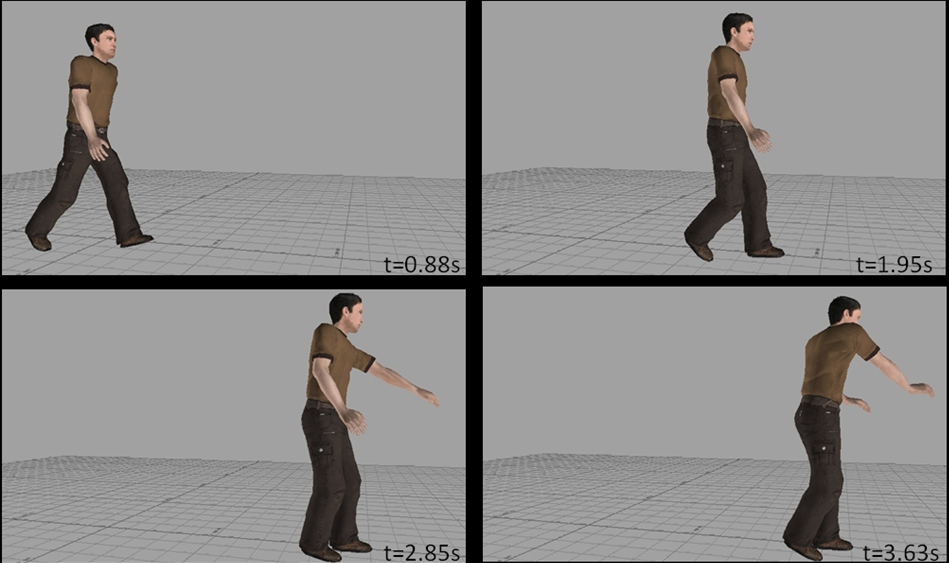
\includegraphics[width=0.5\textwidth]{realavatar.jpg}
  \caption{Illustration of important intermediate postures of the human behavior:
    step with initiation of reaching, standing while opening of drawer, and reaching for the  object.}
\label{fig:real}
\end{figure}

\subsubsection*{Learning of the kinematic primitives}
\label{sc:Modeling}

In order to learn low-dimensional representation of every individual segmented motion we apply the anechoic demixing algorithm \cite{ref:og11, ref:caeg13}.
In this approach the joint angle trajectories are learned unsupervisely as an \emph{anechoic mixture model}: \newline
\begin{displaymath}
\underbrace{\xi_{i}(t)}_{angles}=m_i+\sum_{j}w_{ij}\underbrace{\sigma_{j}\left(t-\tau_{ij}\right)}_{sources}
\end{displaymath}
Here, for each angle trajectory $\xi_{i}(t)$ is represented as the linear mixture of $j$ source signals $\sigma_{j}(t)$ with the linear weights $w_{ij}$
plus the angle mean value $m_i$. 
These source signals can be delayed individually with time delays $\tau_{ij}$, which are different for different angles and source components.
Very good approximations can be computed with less than 4-5 learned source functions \cite{ref:gie09}.
In our standard implementation we first extract the mean angle values from our data.
Then we estimate the weights of additional non-periodic source component, which shape is usually given, but not inferred from the data. 
The shape function serving as nonperiodic source is taken as follows: $s_0(t)=cos(\pi t/T)$, where the time length of trajectory samples (and the period of periodic sources) is $T$.
For the first gait three periodic sources and a non periodic one were sufficient.
For the other two gait, the four sources did not provide a good enough approximation quality.
Therefore additional two sources were learned from the difference between the original trajectories and the learned one using three periodic sources and one non periodic.
Such constrained step-wise approach simplifies the blending between different motion styles, since then the delays of the sources are identical over styles.
The resulting shapes of learned source functions are presented in Fig.~\ref{fig:Sources}.

\begin{figure}[ht]
  \centering
  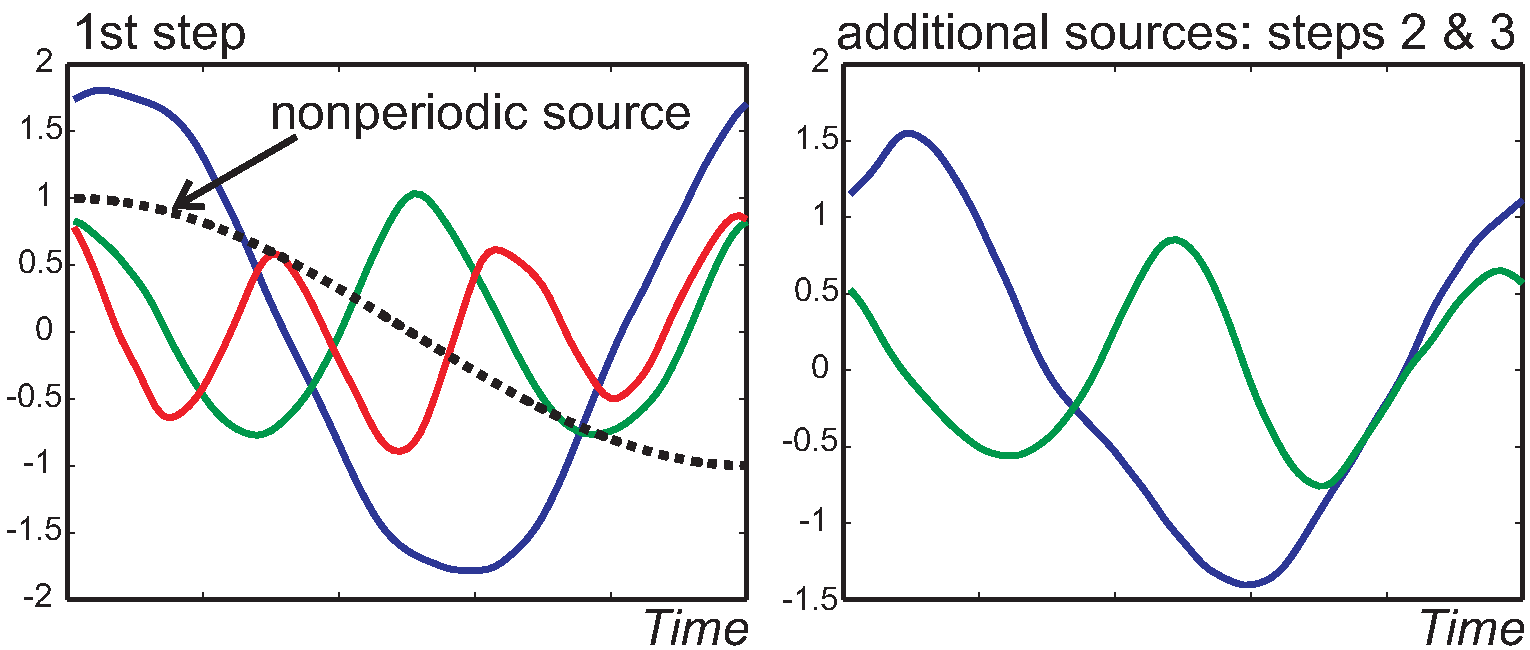
\includegraphics[width=0.48\textwidth]{sources4p2h.pdf}
  \caption{Extracted source signals.}
\label{fig:Sources}
\end{figure}

\subsubsection*{Online kinematic motion synthesis of multi-action sequences}

In order to make the rendering of whole-body trajectories online we propose an architecture built upon the
autonomous dynamical systems regarded as central pattern generators (CPGs), \cite{ref:gie09}. By this approach, our kinematic primitives
are generated online by dynamical systems, or dynamic primitives, DMPs \cite{ref:buc06, ref:inhps13}.
For this we map the solutions of the dynamic primitives onto source signals by Support Vector Regression (using a Radial
Basis Function kernel and the LIBSVM Matlab$^{\circledR}$ library \cite{ref:cha01}). The resulting architecture is summarized at
Fig.~\ref{fig:KinemPrimitivesArchitecture}.

\begin{figure}
  \centering
  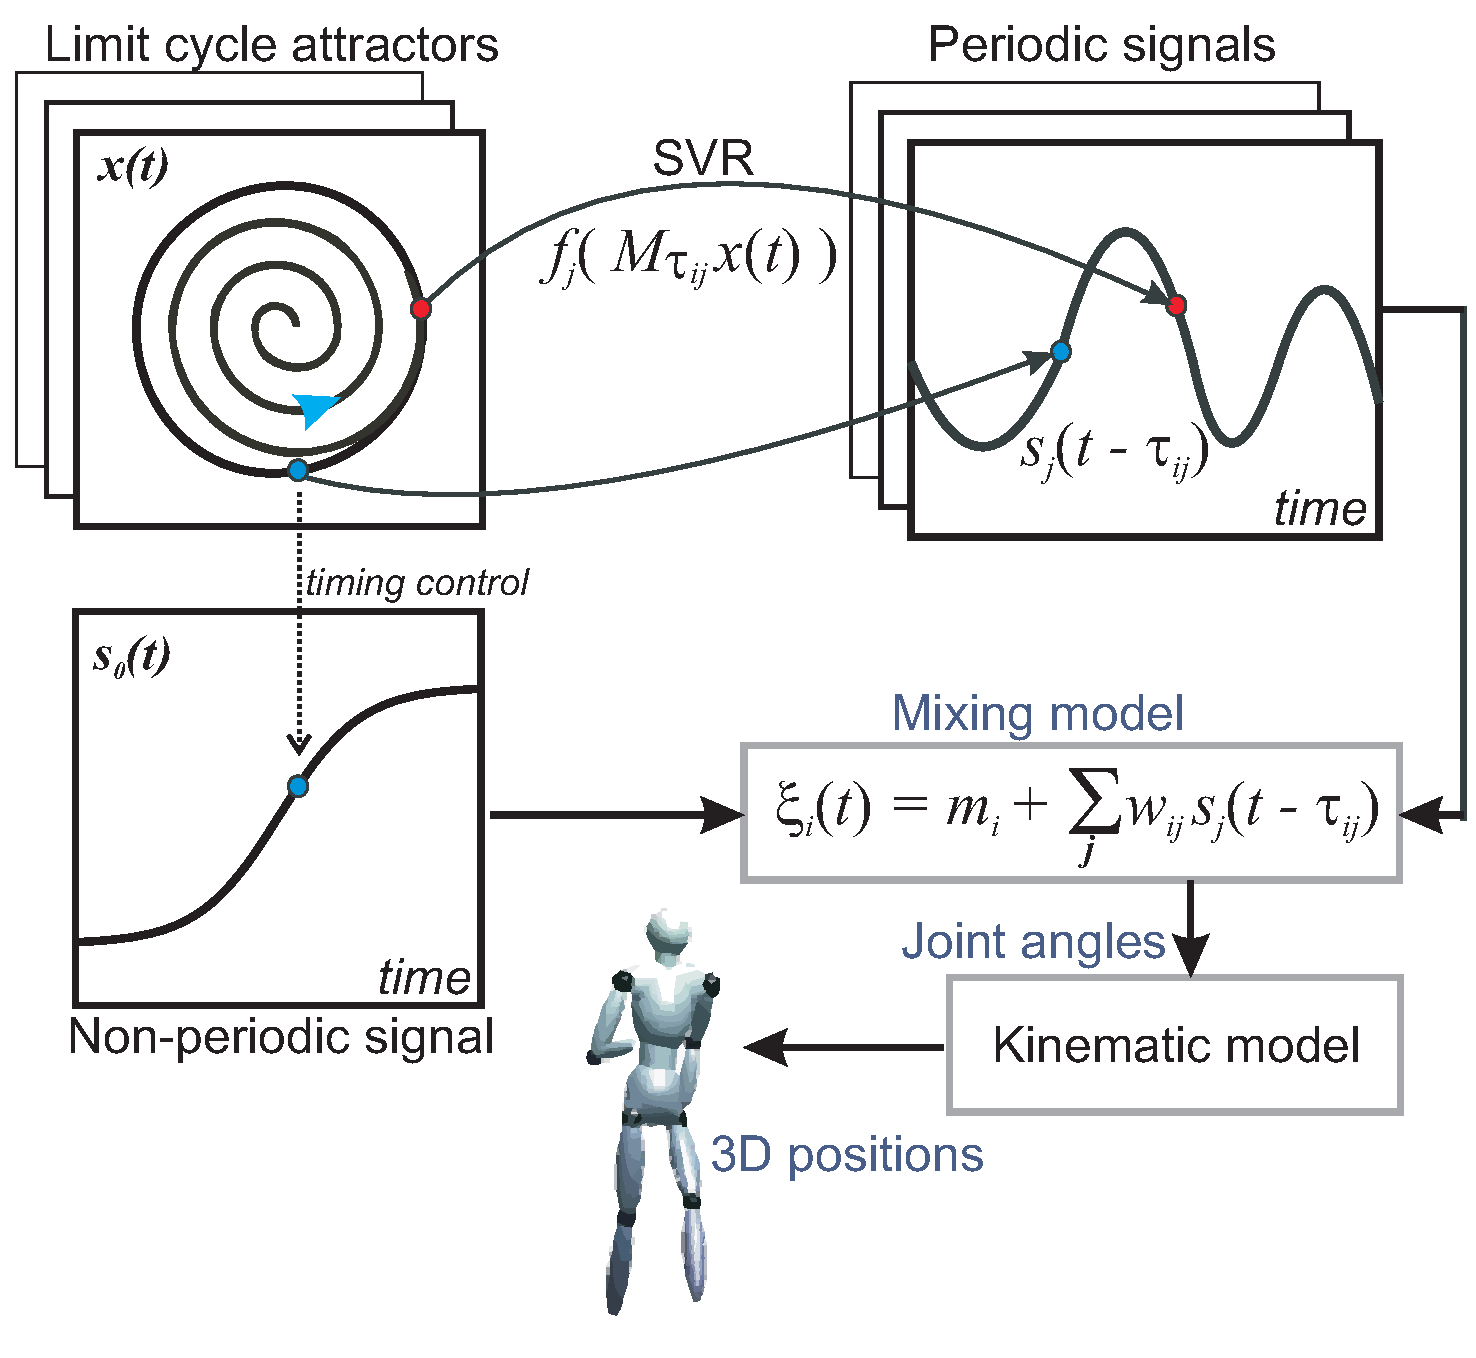
\includegraphics[width=0.48\textwidth]{Graph_syst.pdf}
  \caption{Architecture for the online synthesis of body movements using dynamic primitives, \cite{ref:gie09}. This architecture is fused into one block named \textbf{Kinematic Pattern Synthesis} in Fig.~\ref{fig:onlineWPG} }
\label{fig:KinemPrimitivesArchitecture}
\end{figure}

For the periodic DMPs we chose a limit cycle oscillator (Andronov-Hopf oscillator) as canonical dynamics. It can be characterized by the differential equation system (with $\omega$ defining the eigenfrequency), for the pair of state variables $[x(t),y(t)]$:
\begin{eqnarray*}
\dot{x}(t) =[1-(x^2(t)+y^2(t))]x(t)-\omega y(t)\\
\dot{y}(t) =[1-(x^2(t)+y^2(t))]y(t)+\omega x(t))
\label{hopfosccoupl}
\end{eqnarray*}	
The online phase-shifting is modeled as an additional rotation of the oscillator phase plane, such that, due to the circular shape
of the attractor limit cycle of Andronov-Hopf oscillator, the trajectories on the attractor exhibit simple time-delays, c.f. \cite{ref:gie09}.
The instantaneous phase of the leading DMP also controls the start-triggering event for the non-periodic source. All the periodic DMPs
are phase-coupled in order to assure the coordinated globally stable dynamics. The methods of coupling was designed based on Contraction Theory, \cite{ref:par09}.

To model the actions with variable styles we do learning of nonlinear mappings between task parameters and action parameters (the sources weights).
This mapping is learned by Locally Weighted Linear Regression method (LWLR), \cite{ref:mlsg15}, and the relevant task parameters are steps lengths and timings.
For the synthesis of multi-step step sequences the step lengths are computed from the current estimated target distance. The simplified strategy taken for the
online synthesis is the following: the step lengths in the first action can be modified in range of training data (additional steps can be introduced by higher level
supervision algorithm, if target distance is too large); the step length in the second action is computed to realize maximum comfort distance for reaching. The smooth interpolation between the morphable weights of the kinematic primitives at the moments of concatenation of action is described with all technical details in \cite{ref:mlsg15}.

\subsubsection*{Processing}

\begin{figure}[ht]
  \centering
  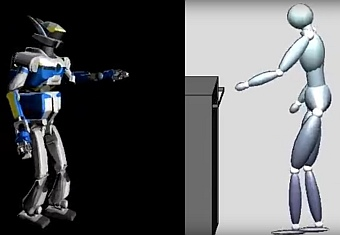
\includegraphics[width=0.36\textwidth]{RobotAvatarjpg2.jpg}
  \caption{The result of the retargeting of the drawer opening task onto the unconstrained skeleton of the HRP-2 robot. The movie is available here [\url{http://tinyurl.com/j8qnbtp}}
\label{fig:RobotHuman}
\end{figure}

Once the recorded motion is learned, it is animated in MotionBuilder (Autodesk),
using an 'actor' puppet whose geometric parameters were adapted to the recorded subject.
The trajectory was first normalized in duration and mapped to the robot using the Denavit-Hartenberg (DH) convention.
The joint limits are not taken into account at this stage.
Fig.~\ref{fig:RobotHuman} is a frame of the movie [\url{http://tinyurl.com/j8qnbtp}.
It shows the animated HRP-2 in MotionBuilder (Autodesk) before kinematic re-targeting.
At this point the trajectory are still not feasible (see Sec.~\ref{sc:Results}).
After that the trajectories are kinematically re-targeted using inverse kinematics and scaled down to fit HRP-2 kinematics and dynamics constraints.
The details of this process is in Sec.~\ref{sc:Results}.
The articular trajectory obtained are then learned using the architecture depicted above and in Fig.~\ref{fig:KinemPrimitivesArchitecture}.

\subsection{Robotics Implementation}
\label{sc:Implementation}

\subsubsection*{Walking pattern generator}

In this application we used the pattern generator described in Chap.~\ref{chap:nmpc} as well.
The interest of this choice is that the lower part of the robot will be driven by the learned human CoM velocity and pelvis rotation.
Moreover the walking pattern generator being a bottom up approach and a well tested algorithm in the humanoid robotic platform HRP-2 at LAAS-CNRS we can warranty the safety of the robot in terms of auto-collision and balance.
The other main advantage is that the implementation include the dynamic filter, often seen as a kind of Newton-Raphson iteration \cite{ref:stasse13}.
In other word we can see the upper body motion as perturbation on the robot dynamic and cancel it via the use of the dynamic filter.
For more detail about the dynamic filter itself the reader is kindly ask to refer to An.~\ref{an:dyn:filter}.

\subsection{Overall architecture}

\begin{figure} [ht]
  \centering
  %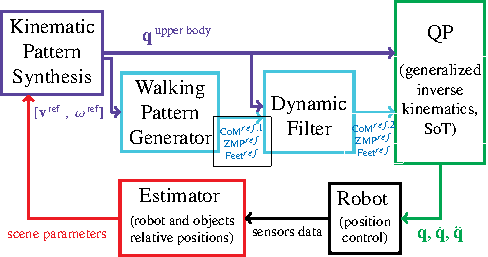
\includegraphics[width=0.6\textwidth]{roboticscheme.pdf}
  %!TEX root = ../../14-icra-RealTimeNMPC.tex

\tikzstyle{block} = [draw=blue!50, fill=blue!20, rectangle,
    minimum height=2em, minimum width=5em, align=center]
\tikzstyle{point} = [coordinate]
\tikzstyle{pinstyle} = [pin edge={to-,thin,black}]

\definecolor{KPS}{RGB}{204 ,  85 , 0}% corail
\definecolor{SBG}{RGB}{222, 152, 22 }% melon
\definecolor{WPG}{RGB}{231 ,  62 , 1}% orange 
\definecolor{SOT}{RGB}{179, 103, 0}% cuivre
\definecolor{ROB}{RGB}{173, 79, 9} % roux
\definecolor{EST}{RGB}{255, 127, 0}

% The block diagram code is probably more verbose than necessary
\begin{tikzpicture}[auto, scale=1.0]
  \draw [fill=green,opacity=.1,text opacity=1] (2.2,1.0) rectangle (14,-2.2);
  \node at(11,-2.0) {\textcolor{green!20!black!100}{Stack of Task}};

    \node [block, text depth=0.7cm, minimum width=2.0cm] at (10.0,-3.0) (robot) {
        Robot
    };
    \node [block, text opacity=1, opacity=0, font=\small, minimum width=1.1cm ] at ([yshift=-0.2cm]robot.center){
      (position \\
      control)
    };
%%%%
    \node [block,  text depth=0.8cm, minimum width=3.0cm] at (5.0,-3.0) (estimator) {
      Estimator 
    };
    \node [block, text opacity=1, opacity=0, draw=white, font=\small, minimum width=1cm ] at ([yshift=-0.2cm]estimator.center){
      (robot and objects\\
      relative positions)
    };
%%%%
    \node [block,  minimum width=0.1cm] at (3.5,-1.0) (wpg) {
        Walking\\
        Pattern\\
        Generator
    };
%%%%
    \node [block,  minimum width=0.1cm, text depth = 0.18cm] at (7.0,-1.0) (dyn) {
        \\[0.1cm]
        Dynamic\\
        Filter
    };
%%%%%
    \node [block,  text depth = 0.7cm, minimum width=2.0cm] at (10.5,-0.5) (sot) {
      \\[0.1cm]
      Task for\\
      Trajectory\\
      Tracking
    };
%%    \node [block, text opacity=1, opacity=0, draw=white, font=\footnotesize, minimum width=1.5cm ] at ([yshift=-0.3cm]sot.center){
%%      (generalized\\
%%      inverse\\
%%      kinematics,\\
%%      SoT)
%    };
    \node [block,  text depth = 1.0cm, minimum width=1.0cm] at (13.1,-0.5) (qp){
      \\[0.5cm]      
      QP\\solver
    };
%%%%  
    \node [block,  minimum width=0.1cm] at (0.0, 0.0) (kps) {
    		Kinematic \\
      Pattern \\
      Synthesis
    	};
%%%%%%%%%%%%%%%%%%%%%%%%%%%%%%%%%%%%%%%%%%%%%%%%%%%%%%%%%%%%%%%%%%%%%%%%%%%%%%%%%%%%%%%%%%
    % PATHS
    	% Forward chaine
    	\node [point] at ([xshift=-0.5cm]wpg.west) (walkingwest) {};
    \draw [ - ] ([yshift=-0.3cm]kps) -| node {} (walkingwest);
    \draw [ ->] (walkingwest) |- node [left] {\small $[{\mathbf v}^{\,{\text{ref}}}\;,\;{\mathbf \omega}^{\,{\text{ref}}}]$} (wpg.west);
%%%%    
    	\node [point] at ( $(dyn.west) + (-0.4,1.0)$ ) (dynwest) {};
    \draw [ - ] ([yshift=+0.1cm]kps) -- node  [above] {\small ${\mathbf q}^{\,{\text{upper body}}}$} (dynwest);
    \draw [ ->] (dynwest) |- node {} ([yshift=+0.3cm]dyn.west);    
    \draw [ ->] (dynwest) |- node {} ([yshift=+0.5cm]sot.west);
%%%%
    \draw [->] ([yshift=-0.1cm]wpg.east) -- node [below , font=\small] {} ([yshift=-0.1cm]dyn.west);
    \node [block, text opacity=1, opacity=0, font=\scriptsize, minimum width=0.01cm] at ($(dyn.west) + (-0.9,-0.7)$){
      CoM$^{ref,{\bf 1}}$ \\ ZMP$^{ref}$ \\ Feet$^{ref}$
    };
%%%%
    \draw [->] (dyn.east) -- node {} ([yshift=-0.5cm]sot.west);
    \node [block, text opacity=1, opacity=0, font=\scriptsize, minimum width=0.01cm] at ($(sot.west) + (-0.9,-1.1)$){
      CoM$^{ref,{\bf 2}}$ \\ ZMP$^{ref}$ \\ Feet$^{ref}$
    };
    
    \draw [draw,->] (sot) -- node {\small Tasks} (qp.west);

   	% Feedback chaine
    	\node [point] at ($(sot.east) + (0.1,0.0)$) (soteast) {};
    \draw [draw,->] (qp) |- node {\small ${\mathbf q},\dot{{\mathbf q}},\ddot{{\mathbf q}}$} (robot);
    
    \draw [draw,->] (robot) -- node {\small sensors data} (estimator);
    
    \draw [draw,->] (estimator) -| node [below right = 0.0cm and 0.5cm]{\small scene parameters} ($(kps.south)+ (-0.1,0.0)$);

    
%%%%%%%%%%%%%%%%%%%%%%%%%%%%%%%%%%%%%%%%%%%%%%%%%%%%%%%%%%%%%%%%%%%%%%%%%%%%%%%%%%%%%%%%5
\end{tikzpicture}


  \caption{This scheme describe the feedback loop used to control the humanoid robot HRP-$2$. With $[{\mathbf{v}}^{ref}, {\mathbf{\omega}}^{ref}]$ as respectively the linear and angular velocity and ${\mathbf{q}}^{upper body}$ the upper body joint trajectories computed from the kinematic pattern synthesis. ${\mathbf q},\dot{{\mathbf q}},\ddot{{\mathbf q}}$ are respectively the generalized position and velocity vectors computed using the Stack of Tasks (SoT).}
\label{fig:onlineWPG}
\end{figure}

In the following we give the brief overview of the proposed robotics platform implementation (see Fig.~\ref{fig:onlineWPG}).
The module labelled 'Kinematic Pattern Synthesis' is the system described in the previous Subsec.~\ref{subsec:modeling}.
This module computes the upper body trajectory and the pelvis linear and angular velocity.
The walking pattern generator than computes the CoP and feet trajectory and send them to the dynamic filter.
In turn, the dynamic filter computes the correction to apply to the CoM dynamics form the CoM, the feet and the upper body trajectories.
The whole body trajectory is then computed by a generalized inverse kinematics using the corrected CoM, the feet, and the upper body articular trajectories.
The framework used is called the 'Stack-of-Task' a.k. SoT.
Once the whole body trajectory computed the robot track them and an estimator evaluates the relevant state of the robot and the scene parameters.
The 'Kinematic Pattern Synthesis' use these data to recompute another set of upper body trajectory and pelvis velocities.
This architecture has not been tested online yet.
However the offline movement ran on HRP-2 indicates that this approach is feasible.
In the next section we will discuss in more details the obtained results during the simulations and experiments.

\section{Results}
\label{sc:Results}

In this section we will discuss the results obtained from experiments.
We will firstly introduce the setup of the experiment, then we will present the first results using the upper body trajectories re-targeted using kinematics.
The discussion will be about the bottom heck of this approach and which possible solution exists.
We will therefore explain in the next paragraph which solution we chose.

\subsection{Experimental setup}

The synthesis architecture described in Sec.~\ref{sc:Implementation} was first tested open loop control in simulation using the OpenHRP simulator and the HRP-2 robot model.
In these simulations, the robot starts from the parking position and makes a transition to a normal step.
At the end of this step the linear and angular pelvis velocities were determined and used as initial conditions.
At the end of the last action a spline interpolation of pelvis angular and positional coordinates was used to change the robots state back to the parking position (introducing
 two additional steps on the spot). A snapshot of the executed behavior is presented in Fig.~\ref{fig:openHRPsim}.
 The drawer was not used here because the robot needs more teaching trajectories to really execute the task.
 In this chapter we show a proof of concept concerning the architecture of control.
 
\begin{figure}[h]
  \begin{center}
    \subfloat[Off-line synthesised trajectories generated with the OpenHRP simulator.]
    {
      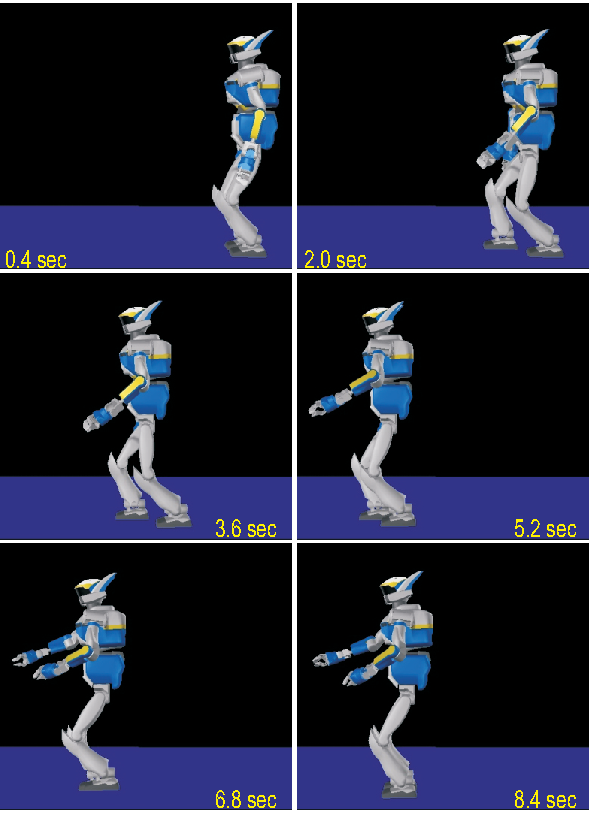
\includegraphics[height=0.5\textwidth]{sim6snapshots.pdf}
      \label{fig:openHRPsim}
    }\hspace*{2cm}
    \subfloat[Real HRP-2 robot performing walking-reaching sequences.]
    {
      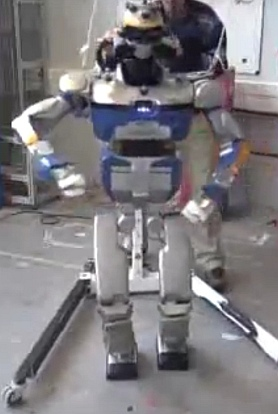
\includegraphics[height=0.5\textwidth]{realhrpwalks.jpg}
      \label{fig:realhrp2walks}
    }
    \caption{Experiment using the HRP-2 in LAAS-CNRS}
    \label{fig:renonculacees}
  \end{center}
\end{figure}

\subsection{Kinematic re-targeting}

As explain above the re-targeting process is divided in two steps, first the human body trajectory are scaled and mapped on the robot joint, and second the inverse kinematics is used to respect kinematic constraints.
This kinematic mapping is not sufficient to make HRP-2 walking.
Indeed we can see in Fig.~\ref{fig:RobotHuman} that the feet are not flat on the ground while satisfying the joint limits.
An additional problems are the numerical singularities and discontinuities in the articular trajectories.
The former forbid the use of stabilizers using fast inverse kinematics like the commercial one implemented on HRP-2 by Kawada.
The latter is incompatible with the dynamic filter as the articular trajectory has to be at least $\mathcal{C}^2$ (see An.~\ref{an:dyn:filter}).

A final point concern the dynamics.
In fact the kinematic re-targeting concern only the kinematics, there are no notion of balance.
This could result in a CoP out of the support polygon.

One possible workaround is to develop an optimization problem taking into account the whole body dynamics, like in \cite{ramos:ram:2015}.
The idea is to find a feasible solution for the upper body knowing the lower body dynamics which is a simple linear inverted pendulum dynamics.
Those trajectories would then be consistent regarding the robot dynamics as well as the closest possible to the referenced human motion.

Another possible workaround is when a good knowledge of the system is available.
One can find a morphing criteria on the trajectory so that the dynamic of the linear pendulum is not too much perturbed.
Usually the heavy body velocities and acceleration heavily impact the robot dynamic.
So scaling the trajectory of these bodies reduce the impact on the dynamic.
This allow the dynamic filter to create dynamically consistent trajectory in only one iteration.


\subsection{Experimental results}

For the experiment the trajectories were re-sampled, resulting
in a normalized duration of 1.6 sec for each action.
The data was split into two subsets, separating
the stored pelvis trajectories and the upper body articular trajectories.
The pelvis position trajectories were rescaled, ensuring the maximally admissible
velocity for the HRP-2 robot (0.5 m/sec).
The pelvis linear and angular velocity was used as input to the walking pattern generator.

For our application we did not implement an optimization problem because of a lack of time.
Indeed designing an optimization problem fast enough to keep the real-time aspect of the architecture is quiet a challenge.
Moreover we just wanted to make a proof of concept regarding the feasibility of the global approach.
From experience we know that HRP-2 main weights are in its waist and chest.
The two bodies are joint with two degrees of freedom, pitch and yaw.
The yaw motion is very problematic as it creates angular momentum around the vertical axis.
In fact, the dynamic filter does not compensate for such momentum.
Hence we decided to scale the yaw angle between the chest and the waist of the robot.
For compensation, a fraction of the yaw-angle trajectory was added back to the trunk yaw-angle.
After this compensation, customized inverse kinematics methods were applied to correct
the upper body arm reaching motion in order to satisfy joint limit constraints.

For the final application on the real robot HRP-2 we filtered the upper body trajectories 
using a Savitzky-Golay Filter.
The result is at least a piece-wize $\mathcal{C}^2$ polynomial trajectories with no time delay.

After training, for the learned parameters, the system generates very natural-looking coordinated three-step
sequences for total goal distances between 2.34 and 2.94 m. This is illustrated by \url{http://tinyurl.com/jtkc6g7}. If the specified goal distance exceeded
this interval, the system automatically introduced additional gait steps, adapting the behavior for goal
distances above 3 meters. \url{http://tinyurl.com/zu55rox}
presents two examples of generated sequences for larger goal distances.

The high degree of real-time online adaptivity is demonstrated in the \url{http://tinyurl.com/hnxluuk}.
When avatar approaches the target, and during the second gait cycle the target jumps away towards a more distant position,
where it can not longer be reached with the originally planned number of steps, the online planning
algorithm automatically introduces an additional steps and adjusts the others, so
that the behavior can successfully be accomplished.

A movie of the full 3-action sequence is presented in \url{http://tinyurl.com/jfda5ql},
 and a movie showing a 4-action sequence can be found in \url{http://tinyurl.com/j7dobcn}.
As final step, the architecture was also tested using the real HRP-2 robot, see Fig.~\ref{fig:realhrp2walks}.

The captured movie of the 3-action sequence realized on the real HRP-2 robot is presented in \url{http://tinyurl.com/hfyhmv6}, and a demo of a 4-action sequence is shown in \mbox{\url{http://tinyurl.com/j52c8dz}}.

%
\subsubsection{Feasible motion}

The experiment has been successfully performed $5$ times in a row.
The forces measured on the vertical axis ($z$) are depicted in Fig.~\ref{fig:zforces}.
The maximum force is less than $700\,N$ which is safe for the robot.
For comparison the robots weight is around $56\,kg$, hence the forces applied to the feet in static posture is : $56*\text{gravity} = 56*9.81 = 549.36\,N$.
The impact forces are less than $20\,\%$ higher than the weight of the robot.
If this ratio is higher than $45\,\%$ the robot force sensors may break.
To summarize, this motion is safe to be performed on our humanoid robot HRP-2.
%
\begin{figure}[ht]
  \begin{center}
      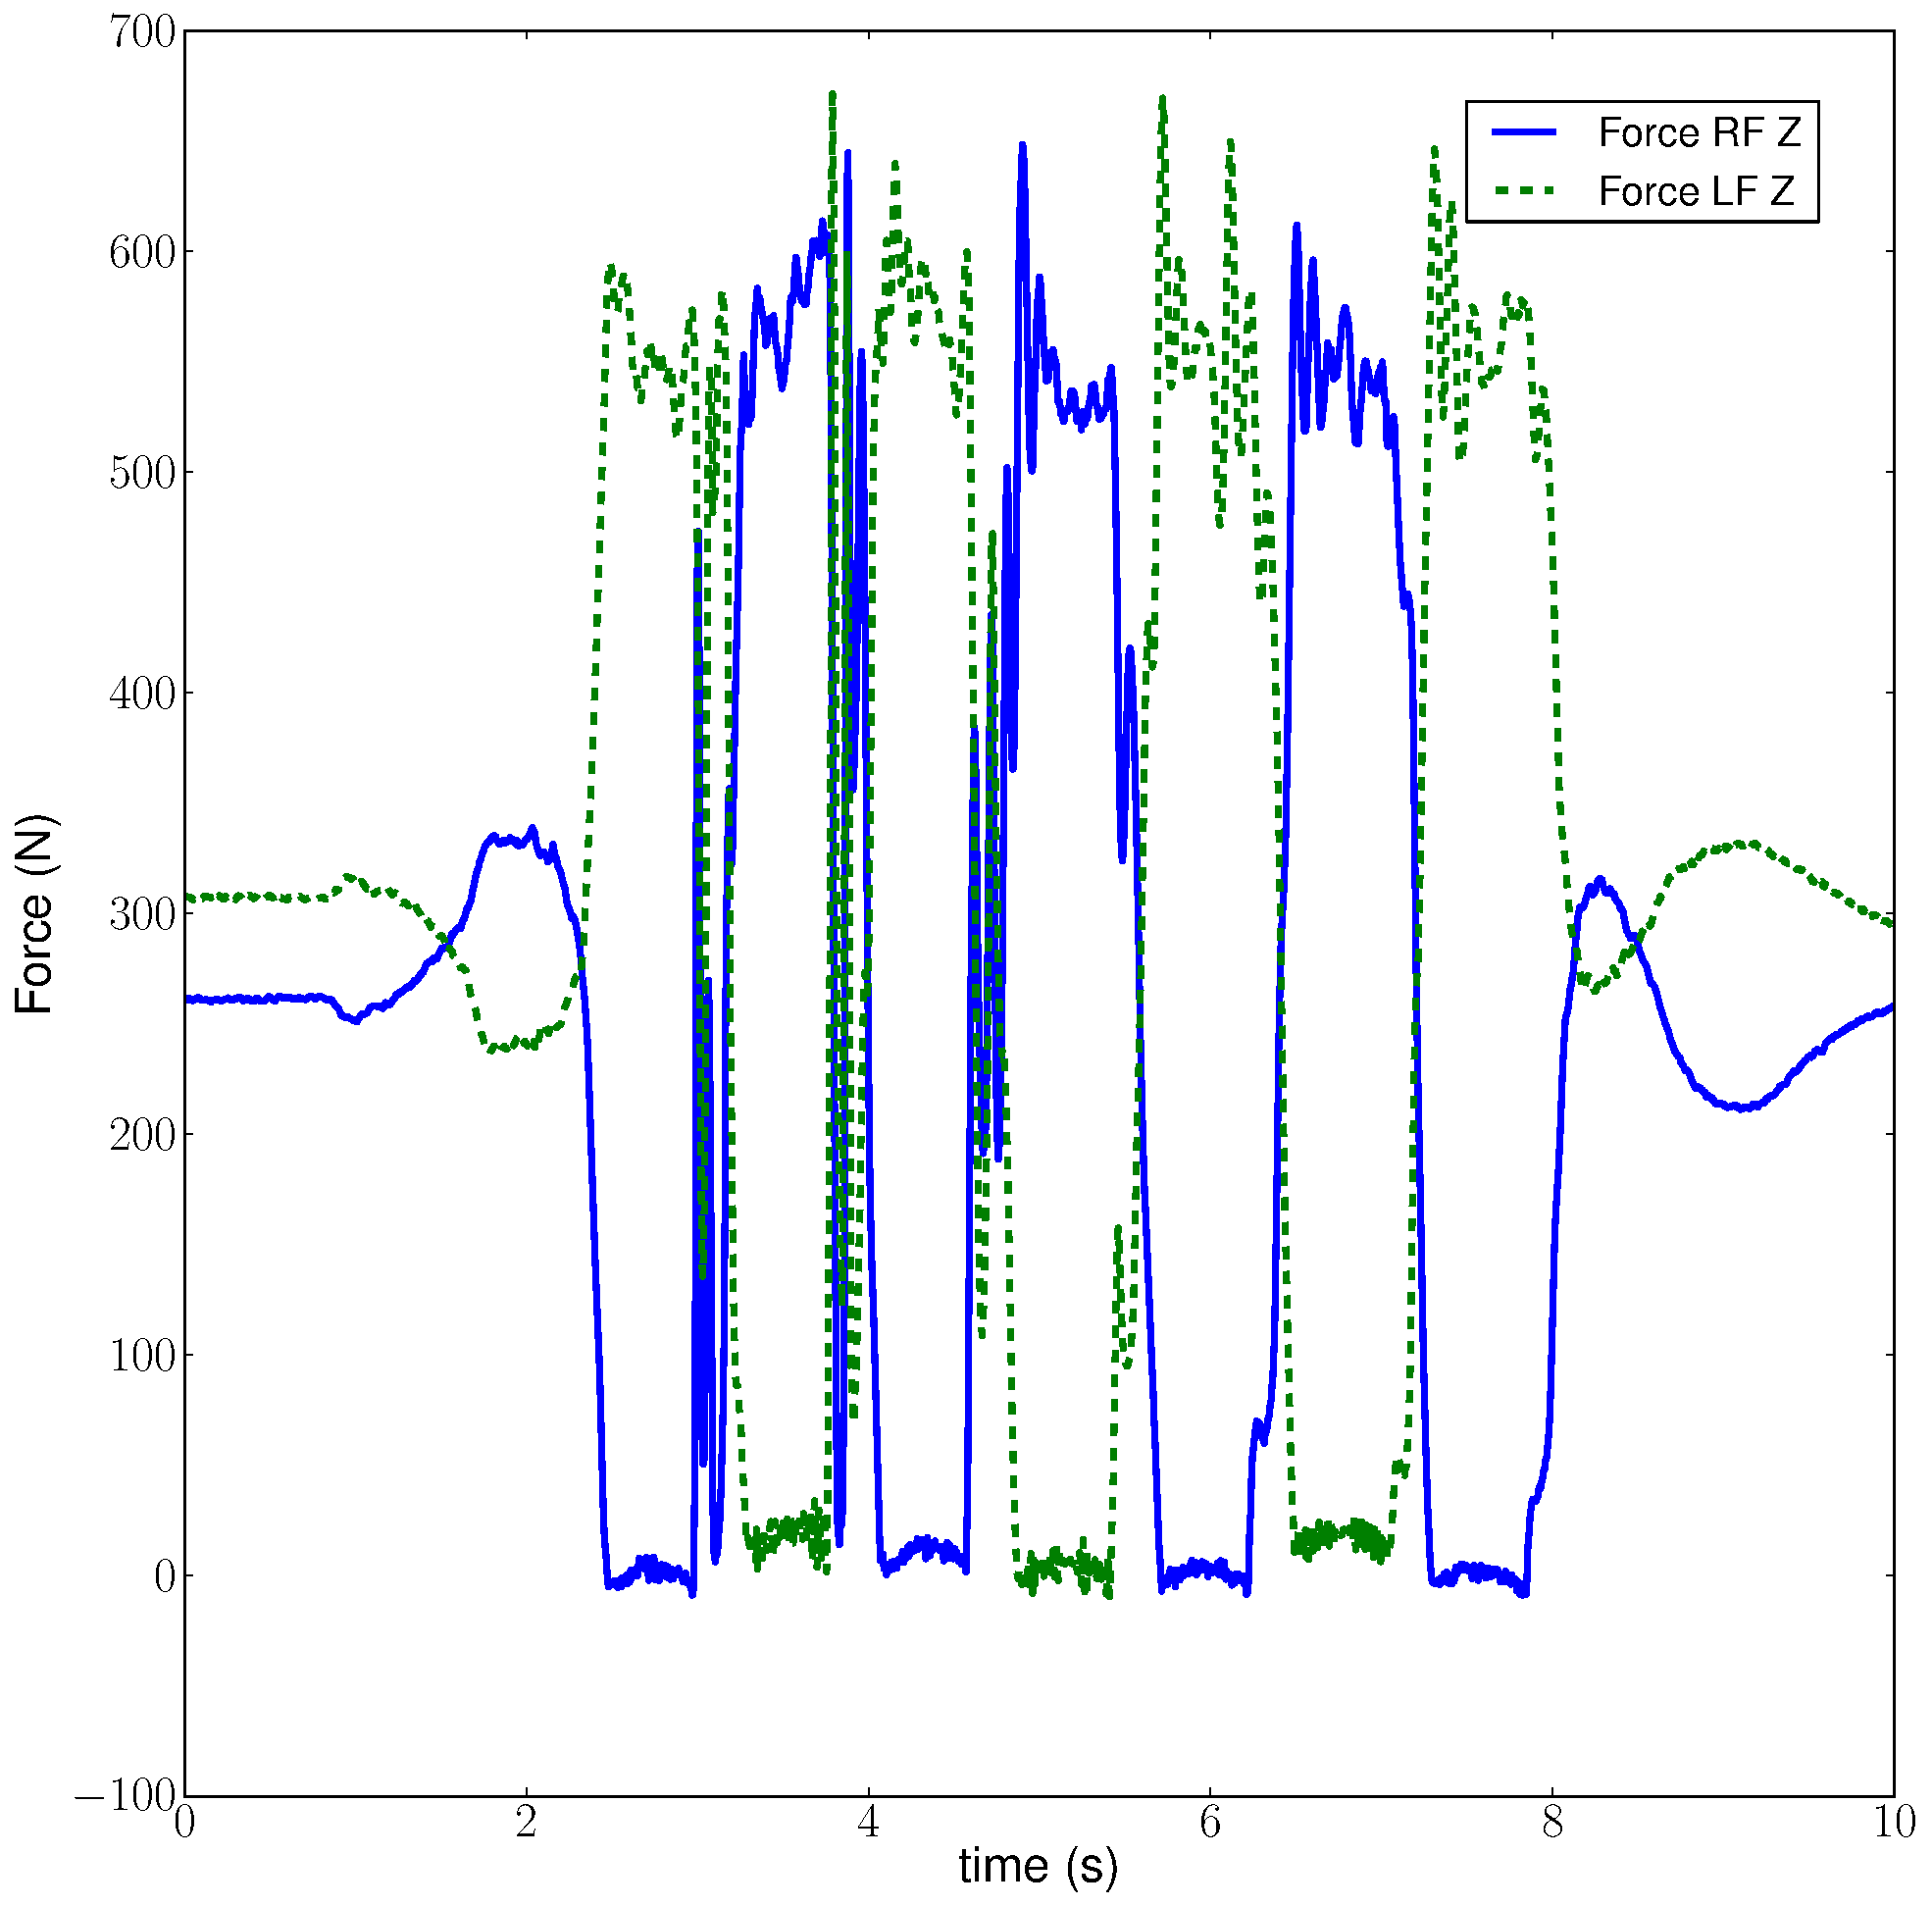
\includegraphics[height=0.6\textwidth , width=0.8\textwidth ]{forcez.pdf}
      \caption{Forces on the vertical axis ($z$) measured during the experiment.}
      \label{fig:zforces}
  \end{center}
\end{figure}
\subsubsection{The role of the dynamic filter}

\begin{figure}[ht]
  \begin{center}
    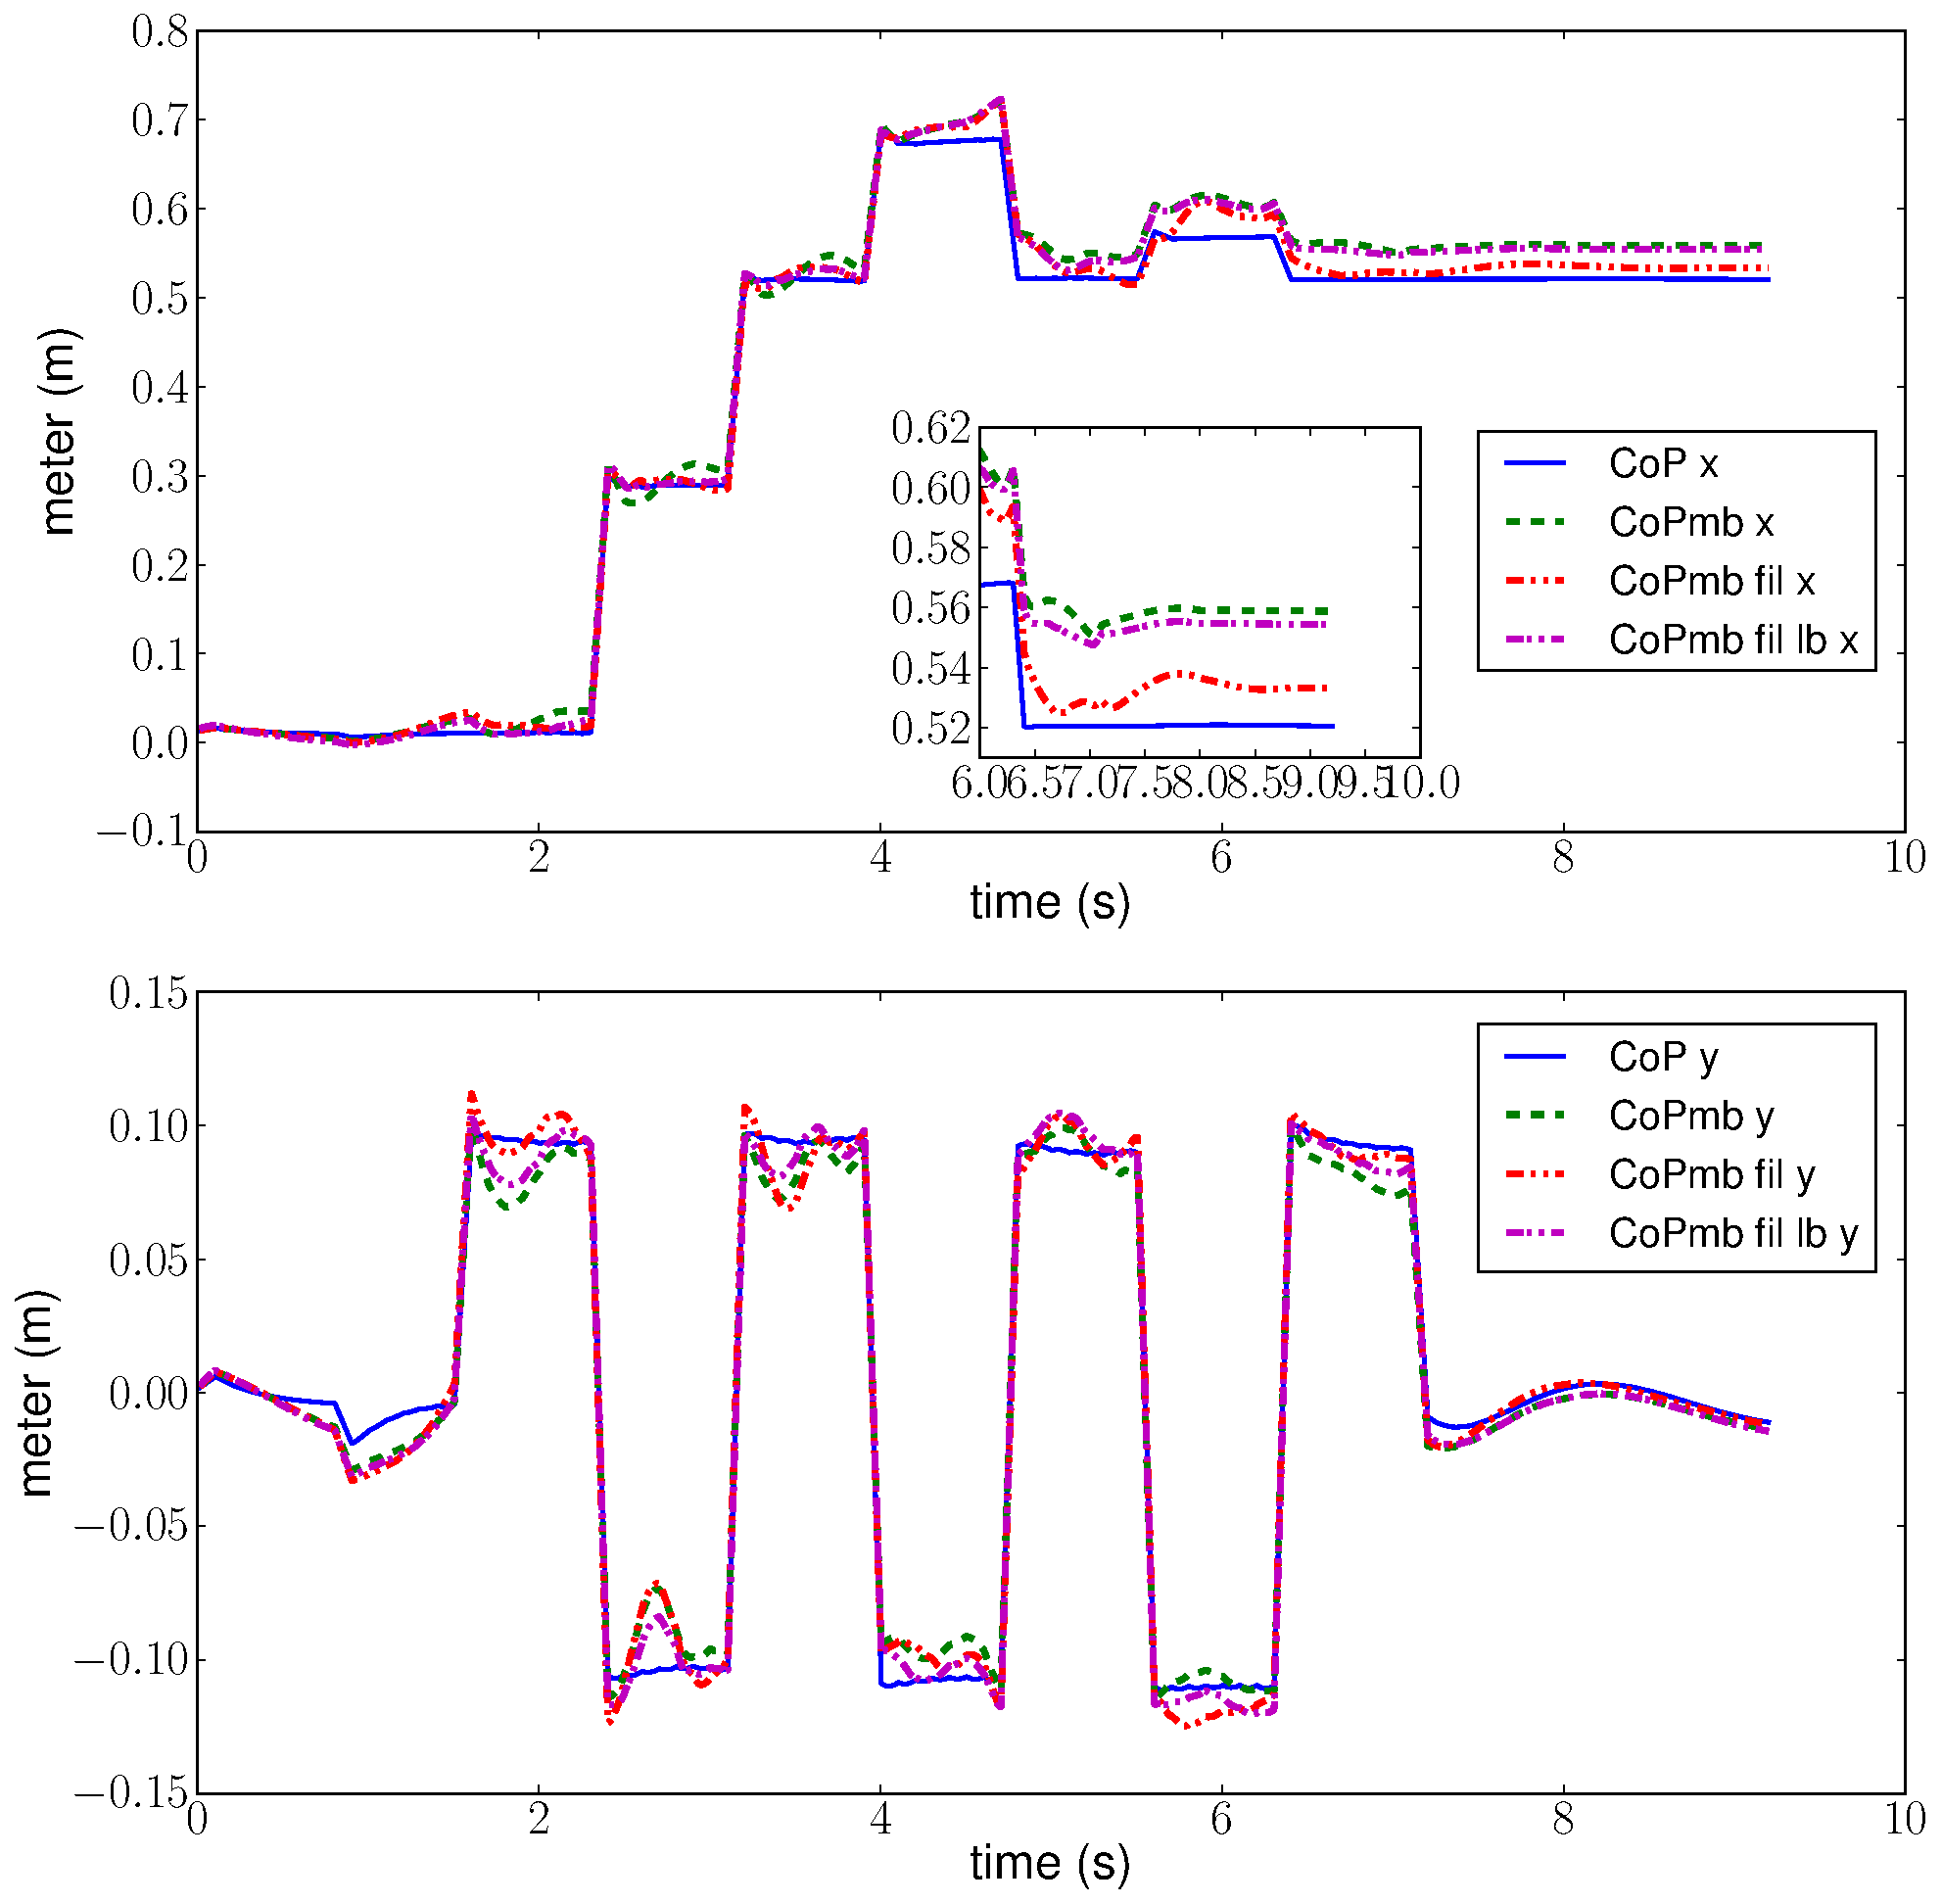
\includegraphics[width=0.65\textwidth, keepaspectratio]{copmb.pdf}
    \caption{These graphs show the theoretical behavior of the CoP. In blue
there is the referenced $CoP$ computed from the linearized inverted pendulum model. In
green you can find the equivalent CoP but computed using the whole body
model. We call it the multibody CoP ($CoP_{mb}$). In red there is the
$CoP_{mb\,fil}$ computed after the dynamic filter correction. And the
magenta line is the CoP with only the lower body filtered
($CoP_{mb\,fil\,lb}$).
In the upper graph a zoom on the end of trajectory shows the efficiency of the dynamic filter.}
    \label{fig:zmpmb}
  \end{center}
\end{figure}
%
In Fig.~\ref{fig:zmpmb} we can see the effect of the dynamic filter on the
$CoP_{mb}$.
The graphs show the comparison between :
\begin{list}{ \arabic{point}.}{%
		\usecounter{point}%
		\setlength{\topsep}{5pt}%
		\setlength{\itemsep}{0pt}%
		\setlength{\parsep}{0pt}%
		\setlength{\labelwidth}{3.em}%
		\setlength{\leftmargin}{2em}%
		\setlength{\labelsep}{0.5em}%
	}
\item[\bluesquare] the referenced CoP computed from the linearized inverse pendulum model ($CoP$, plain blue),
\item[\bluesquare] the CoP computed from the multibody dynamics ($CoP_{mb}$, dotted green),
\item[\bluesquare] the CoP computed from the multibody dynamics after the dynamic filter correction of the whole body ($CoP_{mb\,fil}$, dotted red),
\item[\bluesquare] and the CoP computed from the multibody dynamics after the dynamic filter correction of the lower body only ($CoP_{mb\,fil\,lb}$, dotted magenta).
\end{list}
The first graph represent the trajectories on the sagittal plane (axis $x$).
And the second graph on the coronal plane (axis $y$).

The average and maximum distance between the reference and the non corrected multibody CoP are~:
$$mean ||CoP_{mb}-CoP|| = 0.028 \,m \,,\;\; max ||CoP_{mb}-CoP|| = 0.053 \,m$$
The average and maximum distance between the reference and the corrected multibody CoP are~:
$$ mean ||CoP_{mb\,fil}-CoP|| = 0.015 \,m \,,\;\; max ||CoP_{mb\,fil}-CoP|| = 0.052 \,m$$
Statistically the filtered $CoP_{mb\,fil}$ is closer, in $L_2$ norm, to the
reference than the $CoP_{mb}$
This correction makes the difference between balanced and unbalanced motion.
Indeed we tested the motion using the dynamical filter only for leg motion
(static upper body) and without the dynamic filter in simulation.
In this contexts the robot succeeded to walk until the end of the motion
but fall down when
converging toward a static posture.
In fact the robot arm are lifted to reach the target.
Therefore the center of mass is leaning forward and the CoP comes closer to the foot edges (see the zoom graph in the first graph of the Fig.~\ref{fig:zmpmb}).
The flexibility under the robot soles amplify this phenomena and the CoP goes beyond the
the edge of the feet.
Hence the robot falls.
The maximum errors are not so different.
It is due to the last step forward motion where the robot decelerate and point its arms forward.
The motion itself make the $CoP_{mb}$ moving away from the reference.
The dynamic filter is not able to fully compensate for that much perturbation in a short time.
It will rather decrease the perturbation step by step.
We can see in Fig.~\ref{fig:zmpmb} that at the end the next step ($5\,s$) the $CoP_{mb\,fil}$ (in red) is back to its reference.
As a conclusion, the whole body motion has to be taken into account by the dynamic filter to generate dynamically feasible motions.

\section{Conclusions}
\label{sc:Conclusions}
In this chapter, we have presented an architecture that combines a flexible online
generation of coordinated full-body movements using dynamic movement primitives with a control
architecture that is based on a walking pattern generator, which exploits nonlinear model predictive Control.
The proposed architecture is suitable for the planning of complex coordinated full-body movements in
real-time, and generates dynamically feasible behavior of the robot with appropriate balance
control during walking. The high computation speed distinguishes the proposed framework from
other approaches, which exploit optimum control for the synthesis of dynamically feasible complex
full-body movements.
The functionality and flexibility of the proposed architecture was demonstrated
by simulation using the OpenHRP physics simulator and also on the real HRP-2 robot.

The shown results represent first feasibility tests for this type of architecture. Future work will
have to extend the training sets by inclusion of training sets that maximize the parameter variation
of each individual action, and which include only dynamically feasible behaviors, generated with the
robot simulator. This will make the planned trajectories more similar to dynamically feasible
behaviors and in this way might further increase the flexibility and computational efficiency
of the proposed architecture.
However it is, for the moment, limited to plain ground walking.
As further work we may extend our architecture to multicontact locomotion for humnaoid robots.
This would require the use of another filter for correcting the 3D CoM trajectory.
To our knowledge, no such model predictive control exists yet.
